\section{Auswertung}

\subsection{Zählrohrcharakteristik und Plateauanstieg}

Im ersten Teil des Versuchs befassten wir uns mit der Bestimmung der Zählrohrcharakteristik und der Untersuchung des Plateauanstiegs. Die gemessene Anzahlen an Ereignissen für die jeweilige Zählrohrspannung sind \abbref{plot:bestimmungU0} zu entnehmen.

\begin{figure}[H]
  \centering
  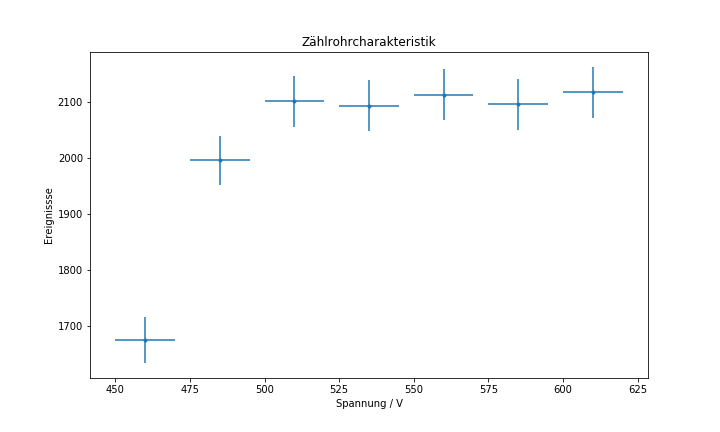
\includegraphics[width=.9\textwidth]{files/bestimmungU0.png}
  \caption{Messung der Zählrohrcharakteristik}
  \label{plot:bestimmungU0}
\end{figure}

Wie bereits in diesem Plot zu erkennen ist, stellt sich ab dem dritten Messpunkt ein plateauartiges Verhalten ein. Wir wählen diesen und die nachfolgenden vier Datenpunkte, um einen linearen Fit durchzuführen, zu sehen in \abbref{plot:bestimmungU0_fit_mean}.

\begin{figure}[H]
  \centering
  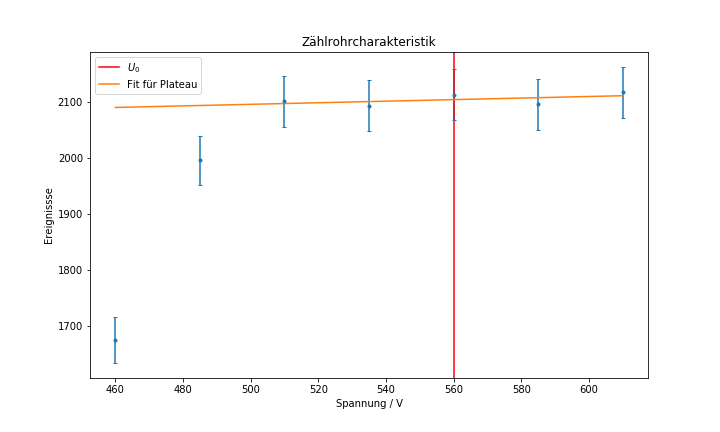
\includegraphics[width=.9\textwidth]{files/bestimmungU0_fit_mean.png}
  \caption{Messung der Zählrohrcharakteristik mit Fit an Plateaubereich}
  \label{plot:bestimmungU0_fit_mean}
\end{figure}

Die Steigung der optimierten Gerade geht gegen 0, was auf den Plateaubereich der Zählrohrcharakteristik hinweist. Die Spannung $U_0$ für den weiteren Versuchsverlauf ermitteln wir als Mittelwert über die fünf Datenpunkte zu $U_0 = 560\si{\volt}$.

Zur Untersuchung des Plateauanstieges nahmen wir bei $U_0$, sowie $U_0 + 100\si{\volt}$ über eine und drei Minuten die folgenden Anzahlen an Ereignissen auf:

\renewcommand{\arraystretch}{1.3}
\begin{table}[H]
  \centering
  \begin{tabular}{c|c|c||c|c|c}
    \diagbox
    {\small t [min]}{\small U [V]} & $U_0$ & $U_0 + 100\si{\volt}$ & $\Delta$ & Anstieg [$\%$] & $\sigma$-Abw.\\\hline
    1 min & $10566 \pm 103$  & $10730 \pm 104$ & $164 \pm 146$ & $1.55 \pm 1.38$ & 1.12 \\\hline
    3 min & $31199 \pm 177$  & $31756 \pm 179$ & $557 \pm 251$& $1.79 \pm 0.8$ & 2.22
  \end{tabular}
  \caption{Anzahl $N$ der Ereignisse zur Untersuchung des Plateauanstiegs}
  \label{tab:plateauanstieg}
\end{table}
\renewcommand{\arraystretch}{1}

In der Tabelle entspricht der Wert $\Delta$ der Differenz 
\begin{gather}
  \Delta = N_{U_0 + 100} - N_{U_0}
  \intertext{mit dem Fehler}
  \sigma_{\Delta} = \sqrt{N_{U_0 + 100} + N_{U_0}}.
  \intertext{Der prozentuale Anstieg ist durch}
  p_{\%} = \frac{N_{U_0 + 100} - N_{U_0}}{N_{U_0}}
  \intertext{mit dem Fehler}
  \Delta p_{\%} = p_{\%} \cdot \sqrt{\qty(\frac{\Delta N_{U_0}}{N_{U_0}})^2 + \qty(\frac{\sigma_{\Delta}}{\Delta})^2}
\end{gather}
gegeben. Die $\sigma$-Abweichung ist durch das Verhältnis $\flatfrac{\Delta}{\sigma_{\Delta}}$ gegeben. Für beide Messzeiten ist der Anstiegt der Anzahl an Ereignissen von $U_0$ zu $U_0 + 100 \si{\volt}$ innerhalb des $3\sigma$-Bereichs und gilt somit als nicht signifikant. 

Nun möchten wir berechnen, wie lange wir hätten messen müssen, um einen prozentualen Fehler $\frac{\sigma_{\Delta}}{\Delta}$ von $1\%$ zu erhalten. Hierzu Betrachten wir zu einer Anzahl $N$ die Zählrate $n = \frac{N}{t}$ pro Sekunde, um folgende Formel herzuleiten:

\begin{align}
 \frac{\sigma_{\Delta}}{\Delta} = \frac{\sqrt{N_{U_0 + 100} + N_{U_0}}}{N_{U_0 + 100} - N_{U_0}} &= \frac{\sqrt{tn_{U_0 + 100} + tn_{U_0}}}{tn_{U_0 + 100} - tn_{U_0}} = \frac{\sqrt{t}}{t} \frac{\sqrt{n_{U_0 + 100} + n_{U_0}}}{n_{U_0 + 100} - n_{U_0}}\\[1em]
 &= \frac{1}{\sqrt{t}} \frac{\sqrt{n_{U_0 + 100} + n_{U_0}}}{n_{U_0 + 100} - n_{U_0}}.
\end{align}
Die Zählraten $n_x$ sind für alle $t$ gleich, somit gilt
\begin{align}
  \frac{\sigma_{\Delta}}{\Delta} \sqrt{t} = \const
\end{align}

Mit dem relativen Fehler, berechnet aus den Werten in Tabelle \ref{tab:plateauanstieg} und der Messzeit $t_{mess}$ von $1 \si{\minute}$ bzw. $3 \si{\minute}$ können wir die Formel wie folgt umstellen
\begin{align}
  \frac{\sigma_{\Delta}}{\Delta}\sqrt{t_{mess}} &= 1\% \cdot \sqrt{t_{1\%}}\\
  \iff  t_{1\%} &= \qty(\frac{\sigma_{\Delta}}{\Delta} \frac{\sqrt{t_{mess}}}{1 \%})^2.
\end{align}

Setzen wir nun die Werte aus Tabelle \ref{tab:plateauanstieg}, so erhalten wir
\begin{align}
  t_{1\%, 1 \si{\minute}} = \qty(\frac{146}{164} \frac{\sqrt{1 \si{\minute}}}{1 \%})^2 = 7917.91 \si{\minute}= 5.50\si{\day}
  \intertext{aus dem Plateauanstieg über $1 \si{\minute}$ und}\\
  t_{1\%, 3 \si{\minute}} = \qty(\frac{251}{557} \frac{\sqrt{3 \si{\minute}}}{1 \%})^2 = 6087.53 \si{\minute} = 4.23\si{\day}
\end{align}
aus dem  Plateauanstieg über $3 \si{\minute}$.

Abschließend zu diesem Versuchsteil möchten wir nun die maximal mögliche prozentuale Variation von $U_0$ zu $U_0 + 100\si{\volt}$ berechnen, wenn wir Anzahlen in einem Vertrauensbereich von $68\%$ und $95\%$ zulassen. Dies entspricht etwa den $1\sigma$- bzw. $2\sigma$-Bereichen.

Den maximalen Anstieg, wenn wir eine Abweichung von $1\sigma$ zulassen erhalten wir durch
\begin{align}
  \Delta_{\max,1\sigma} &= (U_{0+100} + \Delta U_{0+100}) - (U_0 - \Delta U_0)\\[1em]
    &= U_{0+100} + \Delta U_{0+100} - U_0 + \Delta U_0,
\end{align}
lassen also zu, dass $U_0$ um ein $\sigma$ niedriger und $U_{0+100}$ ein $\sigma$ höher ist. Analog gilt für den $2\sigma$-Bereich
\begin{align}
  \Delta_{\max,2\sigma} &= (U_{0+100} + 2 \cdot \Delta U_{0+100}) - (U_0 - 2 \cdot \Delta U_0)\\[1em]
  &= U_{0+100} + 2 \cdot \Delta U_{0+100} - U_0 + 2 \cdot \Delta U_0.
\end{align}
Die prozentuale Variation rechnen wir, wie oben, wieder ausgehend von $U_0$, diesmal aber mit der eingerechneten Abweichung.
\begin{align}
  p_{\%,\max,1\sigma} = \frac{\Delta_{\max,1\sigma}}{U_0 - \Delta U_0}\\[1em]
  p_{\%,\max,2\sigma} = \frac{\Delta_{\max,2\sigma}}{U_0 - 2 \cdot \Delta U_0}.
\end{align}

In diese Formeln können wir nun erneut die Werte aus Tabelle \ref{tab:plateauanstieg} einsetzen und erhalten die in Tabelle \ref{tab:max_sigma_div} aufgezeigten Resultate.

\renewcommand{\arraystretch}{1.3}
\begin{table}[H]
  \centering
  \begin{tabular}{c|c|c}
    \multirow{2}{*}{Messzeit} & \multicolumn{2}{c}{Abweichung im Vertrauensbereich}\\\cline{2-3}
      & $1\sigma \approx 68\%$ & $2\sigma \approx 95\%$\\\hline
      $1\si{\minute}$ & 3.54 \% & 5.57 \% \\\hline
      $3\si{\minute}$ & 2.94 \% & 4.11 \%
  \end{tabular}
  \caption{Mögliche prozentuale Variation der Zählrate im Vertrauensbereich von $68\%$ bzw. $95\%$}
  \label{tab:max_sigma_div}
\end{table}
\renewcommand{\arraystretch}{1}


\newpage\noindent
\subsection{Statistik bei hoher mittlerer Ereigniszahl}

Plot \ref{plot:aufgabe4_data} zeigt die jeweiligen Häufigkeiten, wie oft eine Anzahl an Zerfällen pro Zeiteinheit aufgetreten ist, als Histogramm. Es wurden hierfür 2000 Messungen für Zeitintervalle von $500 \si{\milli\second}$ von einem Computer aufgenommen.

\begin{figure}[H]
  \centering
  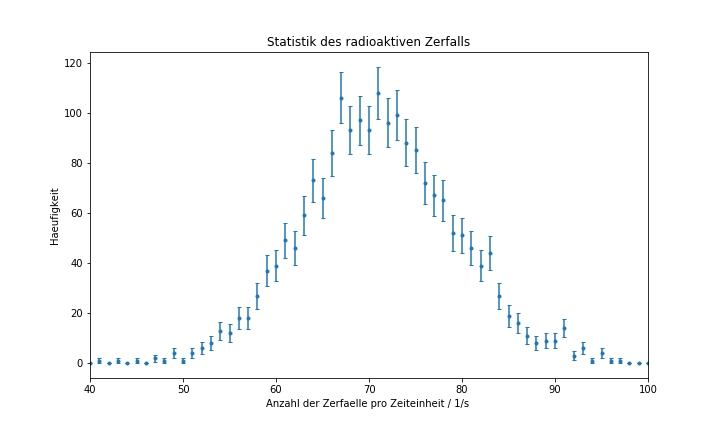
\includegraphics[width=.9\textwidth]{files/aufgabe4_data.png}
  \caption{Verteilung der Zählraten bei hoher mittlerer Ereigniszahl}
  \label{plot:aufgabe4_data}
\end{figure}

Bereits in diesem Plot erkennen wir, dass die Form der Verteilung einer Poisson- oder Gaußverteilung ähnelt. Um dies quantitativ zu untersuchen, werden wir nun an das Histogramm eine Gauß- und eine Poisson-Verteilungsfunktion fitten. Die verwendete Fitmethode verlangt, dass die Fehler gaussverteilt sind, was wir mit einer Einschränkung des Fit-Bereichs auf Klassen mit einer Häufigkeit größer als zehn erreichen. Die Definition der Verteilungsfunktionen ist den Formeln \ref{eq:poisson_distr} und \ref{eq:gauss_distr} des Theorieteils dieser Auswertung zu entnehmen. Als Startparameter für die Fits wählen wir die Werte aus Tabelle \ref{tab:fitting_large_set_start_params}. $\mu$ und $\sigma$ wurden vom Computer bei der Aufzeichnung ermittelt, den Startwert für die Fläche $A$ unter der Kurve entnehmen wir der Praktikumsanleitung.

\renewcommand{\arraystretch}{1.3}
\begin{table}[H]
  \centering
  \begin{tabular}{c|c}
    Parameter & Wert\\\hline
    $\mu$ & 71.05\\
    $\sigma$ & 8.23\\
    $A$ & 2000
  \end{tabular}
  \caption{Startparameter für Gauß- und Poisson-Fit}
  \label{tab:fitting_large_set_start_params}
\end{table}
\renewcommand{\arraystretch}{1}

Plot \ref{plot:aufgabe4_gauss_poisson_fit} zeigt das Ergebnis des Fits, in Tabelle \ref{tab:fitting_large_set_optimized} sind die optimierten Parameter zu finden.

\begin{figure}[H]
  \centering
  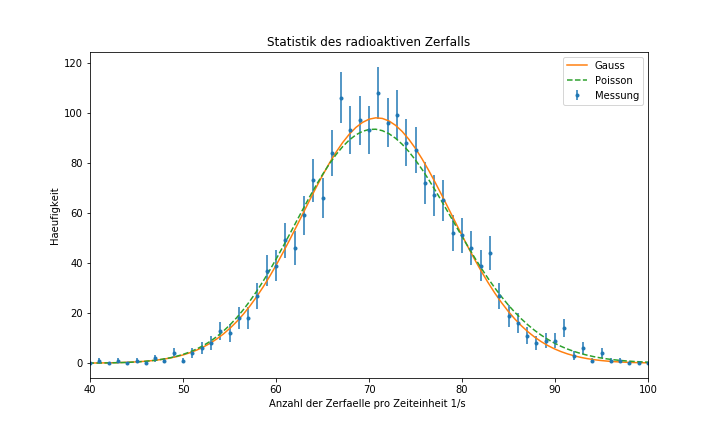
\includegraphics[width=.9\textwidth]{files/aufgabe4_gauss_poisson_fit.png}
  \caption{Verteilung der Zählraten bei hoher mittlerer Ereigniszahl mit Gauß- und Poisson-Fit}
  \label{plot:aufgabe4_gauss_poisson_fit}
\end{figure}

\renewcommand{\arraystretch}{1.3}
\begin{table}[H]
  \centering
  \begin{tabular}{c|c|c}
    \multirow{2}{*}{Parameter} & \multicolumn{2}{c}{Optimierter Wert}\\\cline{2-3}
    & Gauß & Poisson\\\hline
    $\mu$ & $70.86 \pm 0.20$ & $70.96 \pm 0.21$\\
    $\sigma$ & $8.00 \pm 0.18$ & -\\
    $A$ & $1965 \pm 50$ & $1972 \pm 50$
  \end{tabular}
  \caption{Optimierte Werte Gauß- und Poisson-Fit bei hoher mittlerer Ereigniszahl}
  \label{tab:fitting_large_set_optimized}
\end{table}
\renewcommand{\arraystretch}{1}

Zur Beurteilung der Güte des Fits möchten wir nun noch die $\chisq$-Summe berechnen. Hierfür gilt die Formel
\begin{align}
  \chisq = \sum_{i}^{N} \qty(\frac{f(b_i) - h_i}{\Delta h_i})
\end{align}
mit der Anzahl der Messungen $N$, der optimierten Funktion $f$, der Klasse $b_i$, sowie der gemessenen Häufigkeit $h_i$ und Fehler $\Delta h_i$ für die Klasse $b_i$ des Histogramms. Die reduzierte $\chisq$-Summe berechnen wir nach $\chisqrd = \flatfrac{\chi^2}{\mathrm{dof}}$. Den Freiheitsgrad $\texttt{dof}$ bestimmen wir aus der Differenz der Anzahl der Messwerte und der Zahl der Fitparameter.

Für den hier durchgeführten Fit der \underline{Gaußverteilung} erhalten wir die folgenden Werte
\begin{align}
  \chisq &= 18.5, \qquad \chisqrd = 0.5,
  \intertext{für den Fit der \underline{Poisson-Verteilung} die Werte}
  \chisq &= 24.6, \qquad \chisqrd = 0.7.
\end{align}

Betrachten wir die Fläche unter der $\chisq$-Verteilung im Intervall $[\chi_2, \infty]$, so erhalten wir die Wahrscheinlichkeit dafür, dass wir bei einer Wiederholungsmessung einen gleich großen oder größeren $\chisq$-Wert erhalten. Die Fitwahrscheinlichkeiten im betrachteten Fall sind
\begin{align}
  \mathbb{P}(\chisq \geq 18.5) = 99.0\%
  \intertext{für den Gauß-Fit und}
  \mathbb{P}(\chisq \geq 24.6) = 90.0\%
\end{align}
für den Poisson-Fit.

Die Resultate werden im entsprechenden, abschließenden Kapitel diskutiert werden. Nun betrachten wir erst noch die Daten bei kleiner Ereigniszahl.

\subsection{Statistik bei kleiner Ereigniszahl}

Für Intervalle von $100\si{\milli\second}$ wurden in diesem Versuchsteil $5000$ Messungen vom Computer durchgeführt. Die Daten sind im Histogramm \ref{plot:aufgabe5_data} zu sehen.

\begin{figure}[H]
  \centering
  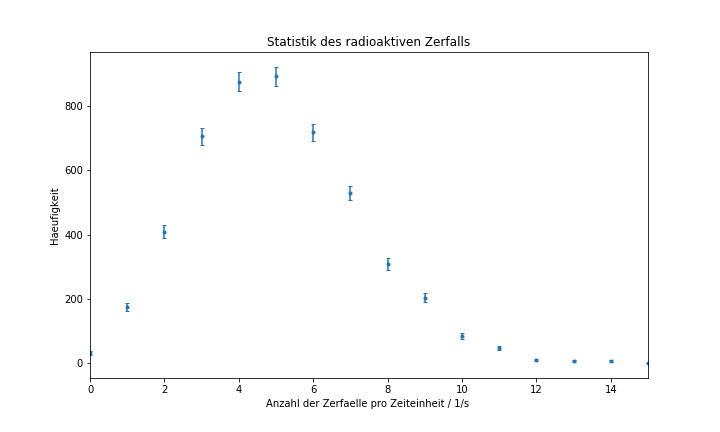
\includegraphics[width=.9\textwidth]{files/aufgabe5_data.png}
  \caption{Verteilung der Zählraten bei kleiner Ereigniszahl}
  \label{plot:aufgabe5_data}
\end{figure}

Bereits hier ist zu erkennen, dass sich die Form der Verteilung eher der einer Poisson-Verteilung annähert. Die Auswertung dieses Versuchsteils läuft analog zur Vorherigen ab. Mit den Startparametern in Tabelle \ref{tab:fitting_small_set_start_params} führen wir Fits für eine Gauß- und eine Poisson-Verteilungsfunktion durch.

\renewcommand{\arraystretch}{1.3}
\begin{table}[H]
  \centering
  \begin{tabular}{c|c}
    Parameter & Wert\\\hline
    $\mu$ & 5.01\\
    $\sigma$ & 2.25\\
    $A$ & 5000
  \end{tabular}
  \caption{Startparameter für Gauß- und Poisson-Fit bei kleiner Ereigniszahl}
  \label{tab:fitting_small_set_start_params}
\end{table}
\renewcommand{\arraystretch}{1}

Die Resultate der Fits sind in \abbref{plot:aufgabe5_gauss_poisson_fit} grafisch dargestellt, die Werte der Parameter können Tabelle \ref{tab:fitting_small_set_optimized} entnommen werden. Es ist zu beachten, dass wir aus Darstellungsgründen im Plot eine logarithmische Skala für die $y$-Achse verwenden.

\begin{figure}[H]
  \centering
  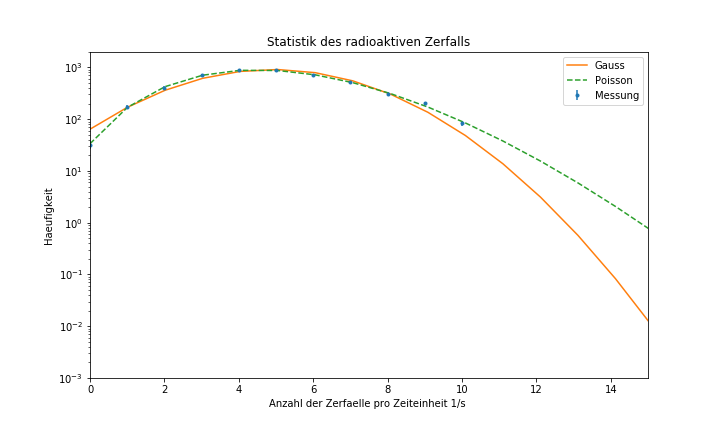
\includegraphics[width=.9\textwidth]{files/aufgabe5_gauss_poisson_fit.png}
  \caption{Verteilung der Zählraten bei kleiner Ereigniszahl mit Gauß- und Poisson-Fit}
  \label{plot:aufgabe5_gauss_poisson_fit}
\end{figure}

\renewcommand{\arraystretch}{1.3}
\begin{table}[H]
  \centering
  \begin{tabular}{c|c|c}
    \multirow{2}{*}{Parameter} & \multicolumn{2}{c}{Optimierter Wert}\\\cline{2-3}
    & Gauß & Poisson\\\hline
    $\mu$ & $4.92 \pm 0.04$ & $5.00 \pm 0.04$\\
    $\sigma$ & $2.134 \pm 0.026$ & -\\
    $A$ & $4880 \pm 71$ & $4992 \pm 72$
  \end{tabular}
  \caption{Optimierte Werte Gauß- und Poisson-Fit bei kleiner Ereigniszahl}
  \label{tab:fitting_small_set_optimized}
\end{table}
\renewcommand{\arraystretch}{1}

Wie zuvor berechnen wir nun auch noch die $\chisq$-Werte, sowie die Fitwahrscheinlichkeiten. Für den Gauß-Fit gilt
\begin{align}
  \chisq &= 94.3, \qquad \chisqrd = 11.9, \qquad \mathbb{P}(\chisq \geq 94.3) = 0.0\%
  \intertext{und für den Poisson-Fit}
  \chisq &= 5.14, \qquad \chisqrd = 0.57, \qquad \mathbb{P}(\chisq \geq 94.3) = 82.0\%.
\end{align}

Auch diese Ergebnisse werden wir im folgenden Kapitel diskutieren.